\documentclass[unicode,10pt,a4paper,oneside,numbers=endperiod,openany]{scrartcl}
\usepackage{tikz}
\usepackage{pgfplots}
\usepgfplotslibrary{colorbrewer} % better colors
\pgfplotsset{compat=1.18}
\usepackage{amsmath}
\usepackage{url}
\usepackage{xcolor}
\usepackage{subcaption}
\usepackage{listings}
\usepackage{multirow}
\lstdefinestyle{grayverbatim}{
  basicstyle=\ttfamily,%
  backgroundcolor=\color{gray!10},%
  frame=single,%
  framesep=3pt,%
  breaklines=true,%
  columns=fullflexible%
  numberstyle = \tiny,%
  stepnumber = 1,%
  numbersep = 5pt,%
  numbers = left%
}
\definecolor{lightbluehighlight}{RGB}{204,232,255}
\input{assignment.sty}

\begin{document}


\setassignment
\setduedate{27 April 2026, 18:00~(Europe/Zurich)}

\serieheader{High-Performance Computing Lab for CSE}{2026}
            {Student: Riccardo Polo}
            {Discussed with: Giovanni Guidarini}
            {Report for Project 4}{}
\newline

% you may comment this for the final submission, but make sure to comply with
% the policy
\assignmentpolicy

\newpage
\section{Computing $\pi$ with MPI [10 points]}
%\input{sections/01_pi.tex}
\subsection{Parellization using MPI}
The parellel implementation of the $\pi$ computation is based on the idea of dividing the interval $[0, 1]$ into $N$ subintervals, where $N$ is the number of processes. Each process computes the contribution to $\pi$ from its assigned subinterval and then all contributions are summed together using MPI. In listing \ref{lst:pi_mpi} we show the implementation of the parallel $\pi$ computation using MPI.

\begin{lstlisting}[style=grayverbatim, caption={Parallel $\pi$ computation using MPI}, label={lst:pi_mpi}]
MPI_Init(&argc, &argv);
MPI_Comm_rank(MPI_COMM_WORLD, &rank);
MPI_Comm_size(MPI_COMM_WORLD, &size);

h = 1.0 / (double)N;

MPI_Barrier(MPI_COMM_WORLD);
time_start = walltime();

for (uint64_t i = (uint64_t)rank; i < N; i += (uint64_t)size) {
    double x = (i + 0.5) * h;
    local_sum += 4.0 / (1.0 + x * x);
}

MPI_Reduce(&local_sum, &sum, 1, MPI_DOUBLE, MPI_SUM, 0, MPI_COMM_WORLD);
double time = walltime() - time_start;
if (rank == 0) {
    pi = sum * h;
    printf("# pi N procs time [secs]\n");
    printf("%.15f %20" PRIu64 " %3d %.8f\n", pi, N, size, time);
    }

MPI_Finalize();
\end{lstlisting}
Each process starts from its rank and iterates over the indices of the subintervals assigned to it by incrementing the index by the total number of processes in each iteration. This way, each process computes the contribution to $\pi$ from its assigned subintervals without overlap. After the local sums are computed, they are reduced to a single sum using \texttt{MPI\_Reduce}, which is then used to compute the final value of $\pi$ on the root process (rank 0).

\subsection{Strong scaling}
To evaluate the strong scaling of the parallel $\pi$ computation, we run the program with a fixed problem size $N$ and varying number of processes. The results are shown in figure ~\ref{fig:strong_scaling}, where we plot the speedup achieved by the parallel implementation compared to the serial version.

\begin{figure}[ht]
        \centering
        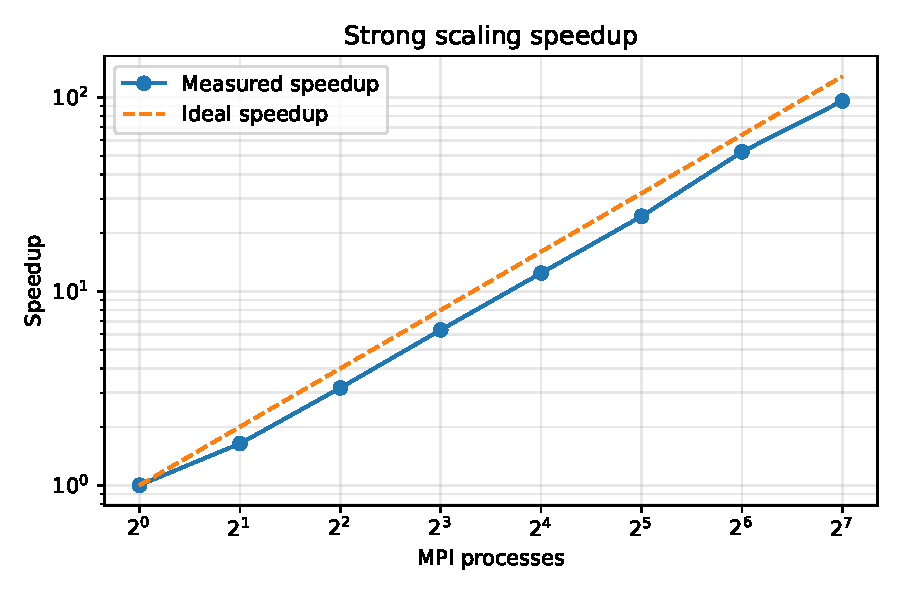
\includegraphics[scale=0.6]{../01_pi/figures/strong_scaling_speedup.pdf}
        \caption{Strong scaling speedup of the parallel $\pi$ computation. Obtained with $N=10^9$.}
        \label{fig:strong_scaling}
\end{figure}

\begin{table}[!h]
\centering
\caption{Strong scaling results using the OpenMP reduction clause ($N=10^9$).}
\label{tab:strong_scaling_reduction}
\begin{tabular}{ccc}
\hline
Threads & Speedup \\
\hline
1   & 1.00 \\
2   & 1.84 \\
4   & 3.26 \\
8   & 6.39 \\
16  & 8.86 \\
32  & 17.66 \\
64  & 31.06 \\
\hline
\end{tabular}
\end{table}
The strong scaling results obtained with MPI show a near-linear increase in speedup for a small number of processes, closely following the ideal trend. As the number of processes increases, the measured speedup progressively deviates from the ideal curve, highlighting the impact of communication overhead and reduced computational workload per process. Nevertheless, the scalability remains good, reaching a speedup close to 100 with 128 processes.\\

Comparing these results with the OpenMP reduction implementation in Table~\ref{tab:strong_scaling_reduction}, we observe a very similar scaling behavior. Both approaches exhibit efficient parallelization at low to moderate parallelism and a loss of efficiency at higher core counts. However, OpenMP achieves slightly better efficiency at comparable core counts, likely due to the shared-memory model which avoids explicit communication overhead.


\subsection{Weak scaling}
The results of the weak scaling tests are shown in figure ~\ref{fig:weak_scaling_efficiency}, where we plot the weak scaling efficiency as a function of the number of processes.\\

The weak scaling efficiency remains high across all tested configurations, staying close to the ideal value of 1. This indicates that the workload is well balanced among MPI processes and that the parallelization strategy is effective.\\

A slight degradation in efficiency is observed as the number of processes increases, particularly at the highest core counts. This behavior is expected and can be attributed to increasing communication overhead and synchronization costs, which become more significant as more processes are involved.
\begin{figure}[ht]
    \centering
    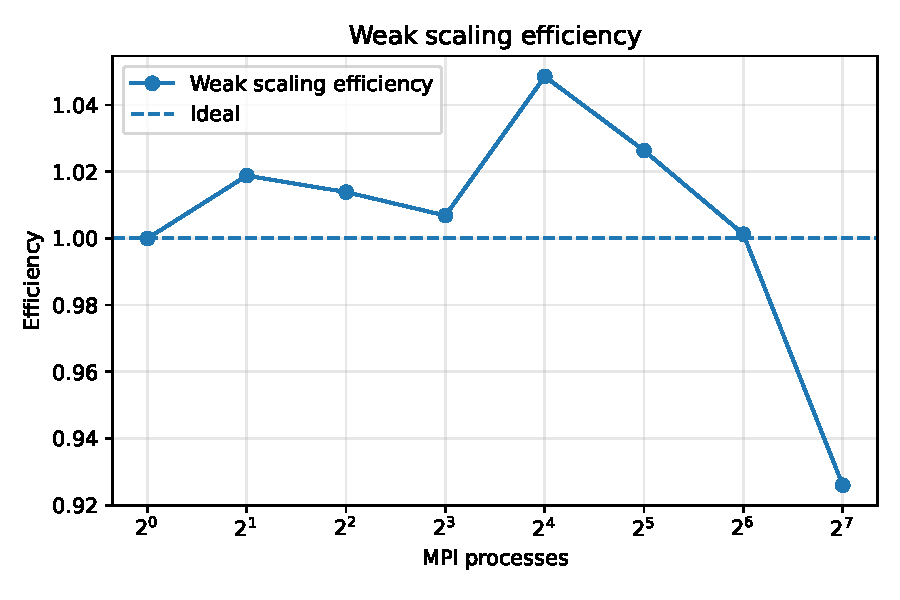
\includegraphics[scale = 0.6]{../01_pi/figures/weak_scaling_efficiency.pdf}
    \caption{Weak scaling efficiency of the parallel $\pi$ computation.}
    \label{fig:weak_scaling_efficiency}
\end{figure}

\newpage
\section{Ring sum using MPI [10 points]}
In listing \ref{lst:ring_sum} we show the implementation of the ring sum using MPI.
\begin{lstlisting}[style=grayverbatim, caption={Ring sum using MPI}, label={lst:ring_sum}]
int main(int argc, char *argv[]) {
int size, rank;
  MPI_Init(&argc, &argv);
  MPI_Comm_size(MPI_COMM_WORLD, &size);
  MPI_Comm_rank(MPI_COMM_WORLD, &rank);

  int send_to   = (rank + 1) % size;
  int recv_from = (rank - 1 + size) % size;

  int sum = rank;       
  int value = rank;     
  int recv_value;

  for (int i = 0; i < size - 1; i++) {
    MPI_Sendrecv(&value, 1, MPI_INT, send_to, 0,
                 &recv_value, 1, MPI_INT, recv_from, 0,
                 MPI_COMM_WORLD, MPI_STATUS_IGNORE);

    sum += recv_value;   
    value = recv_value;  
  }

  printf("Process %d: Sum = %d\n", rank, sum);

  MPI_Finalize();
  return 0;
}
\end{lstlisting}
We implemented the ring sum algorithm using a one-dimensional circular topology, where each process communicates with two neighbors: the next process in increasing rank direction and the previous one, defined respectively as $(\text{rank}+1) \bmod P$ and $(\text{rank}-1+P) \bmod P$, where $P$ is the number of processes.\\

Each process initializes a local accumulator with its own rank and a separate variable containing the value to be propagated through the ring. At every iteration, a process sends its current value to the right neighbor and simultaneously receives a value from the left neighbor. The received value is added to the local sum and then forwarded in the next iteration. After $P-1$ iterations, each process has received all other ranks exactly once, thus computing the global sum.\\

To avoid potential deadlock issues, we used the \texttt{MPI\_Sendrecv} routine, which combines sending and receiving into a single operation. This ensures that all processes can safely exchange messages without the risk of circular waiting that may arise when using separate blocking \texttt{MPI\_Send} and \texttt{MPI\_Recv} calls. The communication pattern is therefore fully synchronized and deadlock-free.

Finally, all processes obtain the same result, confirming the correctness of the implementation as one can see from the output shown in listing \ref{lst:ring_output}.
\begin{lstlisting}[style=grayverbatim, caption={Output of ring sum}, label={lst:ring_output}]
Process 1: Sum = 6
Process 0: Sum = 6
Process 2: Sum = 6
Process 3: Sum = 6
\end{lstlisting}

\newpage
\section{Cartesian domain decomposition and ghost cells exchange [20 points]}

\subsection{Cartesian 2D communicator}
In listing \ref{lst:cartesian_comm} we show the implementation of the Cartesian 2D communicator using MPI.
\begin{lstlisting}[style=grayverbatim, caption={Cartesian 2D communicator using MPI}, label={lst:cartesian_comm}]
int rank, size, i, j, dims[2], periods[2], rank_north, rank_south, rank_west, rank_east;
double data[DOMAINSIZE*DOMAINSIZE];
MPI_Request request;
MPI_Status status;
MPI_Comm comm_cart;
MPI_Datatype data_ghost;

dims[0]= 3;
dims[1]= 4;
periods[0]= 1;
periods[1]= 1;

MPI_Cart_create(MPI_COMM_WORLD, 2 ,dims , periods , 0 , &comm_cart);

MPI_Cart_shift(comm_cart, 1, 1, &rank_south, &rank_north);
MPI_Cart_shift(comm_cart, 0, 1, &rank_west, &rank_east);
\end{lstlisting}

The code first defines the Cartesian topology of the process grid by setting
\texttt{dims[0] = 3} and \texttt{dims[1] = 4}, corresponding to a $3 \times 4$
decomposition. The array \texttt{periods} is set to 1 in both directions, meaning that the topology is periodic both horizontally and vertically: processes at one boundary are connected to processes on the opposite boundary. This implements the cyclic communication pattern required by the exercise.\\

The call to \texttt{MPI\_Cart\_create} constructs a new communicator, \texttt{comm\_cart}, in which all processes are arranged according to this two-dimensional Cartesian topology. Using a Cartesian communicator makes neighbor discovery much simpler than manually computing ranks.\\

The two calls to \texttt{MPI\_Cart\_shift} are then used to determine the ranks of the neighboring processes in the two coordinate directions. In particular, the first call identifies the south and north neighbors, while the second call identifies the west and east neighbors.

\subsection{Derived data type for column boundary}
In listing \ref{lst:derived_type} we show the implementation of the derived data type for column boundary using MPI.
\begin{lstlisting}[style=grayverbatim, caption={Derived data type for column boundary using MPI}, label={lst:derived_type}]
MPI_Type_vector(SUBDOMAIN, 1, DOMAINSIZE, MPI_DOUBLE, &data_ghost);
MPI_Type_commit(&data_ghost);
\end{lstlisting}

The ghost-cell exchange in the horizontal direction involves non-contiguous memory, because a column of the local two-dimensional array is stored with a stride equal to
\texttt{DOMAINSIZE}. To communicate such a column efficiently, a derived MPI datatype is created with \texttt{MPI\_Type\_vector}.\\

This datatype describes \texttt{SUBDOMAIN} elements of type \texttt{MPI\_DOUBLE}, with one element taken from each row and a spacing of \texttt{DOMAINSIZE} elements between successive entries. In this way, the datatype represents exactly one column of the local subdomain. After its definition, \texttt{MPI\_Type\_commit} makes the
datatype available for communication.\\

\subsection{Exchange ghost cells}
In listing \ref{lst:ghost_exchange} we show the implementation of the ghost cells exchange using MPI.
\begin{lstlisting}[style=grayverbatim, caption={Ghost cells exchange using MPI}, label={lst:ghost_exchange}]
/* send top interior row (j = SUBDOMAIN) to north, receive bottom ghost row (j = 0) from south */
    MPI_Sendrecv(&data[SUBDOMAIN + 1 * DOMAINSIZE], 1, data_ghost,
                 rank_north, 0,
                 &data[0 + 1 * DOMAINSIZE], 1, data_ghost,
                 rank_south, 0,
                 comm_cart, MPI_STATUS_IGNORE);

    /* send bottom interior row (j = 1) to south,
       receive top ghost row (j = SUBDOMAIN+1) from north */
    MPI_Sendrecv(&data[1 + 1 * DOMAINSIZE], 1, data_ghost,
                 rank_south, 1,
                 &data[(SUBDOMAIN + 1) + 1 * DOMAINSIZE], 1, data_ghost,
                 rank_north, 1,
                 comm_cart, MPI_STATUS_IGNORE);


    /* send right interior column (i = SUBDOMAIN) to east,
       receive left ghost column (i = 0) from west */
    MPI_Sendrecv(&data[1 + SUBDOMAIN * DOMAINSIZE], SUBDOMAIN, MPI_DOUBLE,
                 rank_east, 2,
                 &data[1 + 0 * DOMAINSIZE], SUBDOMAIN, MPI_DOUBLE,
                 rank_west, 2,
                 comm_cart, MPI_STATUS_IGNORE);

    /* send left interior column (i = 1) to west,
       receive right ghost column (i = SUBDOMAIN+1) from east */
    MPI_Sendrecv(&data[1 + 1 * DOMAINSIZE], SUBDOMAIN, MPI_DOUBLE,
                 rank_west, 3,
                 &data[1 + (SUBDOMAIN + 1) * DOMAINSIZE], SUBDOMAIN, MPI_DOUBLE,
                 rank_east, 3,
                 comm_cart, MPI_STATUS_IGNORE);
\end{lstlisting}

This part of the code performs the exchange of ghost cells with the four neighboring processes of the Cartesian grid. The communication is split into four steps, one for
each boundary: north, south, east, and west. In each case, the interior boundary of the local subdomain is sent to the corresponding neighbor, while the matching ghost layer is received from the opposite side.\\

The first two \texttt{MPI\_Sendrecv} calls handle the exchange in the vertical direction. The top interior boundary is sent to the north neighbor and the bottom ghost layer is received from the south neighbor. Similarly, the bottom interior boundary is sent to the south neighbor and the top ghost layer is received from the north neighbor. Because the domain is periodic, these communications also work correctly for processes located at the physical boundaries of the global domain.\\

The last two \texttt{MPI\_Sendrecv} calls handle the exchange in the horizontal direction. Here the communication involves columns, so the memory layout must be treated carefully. One boundary column is exchanged with the east and west neighbors,
and the received values are stored in the corresponding ghost columns.\\

The use of \texttt{MPI\_Sendrecv} is particularly important because it avoids possible deadlock issues that could arise if all processes tried to perform blocking send operations before posting matching receives. By combining send and receive into one single communication call, the ghost-cell exchange is both safe and simple to implement.\\

The output is shown in listing \ref{lst:ghost_output}.\\
From it one can see the ranks of the neighboring processes and the data array after the ghost cell exchange, confirming that the communication was successful and that the ghost cells have been updated with the correct values from the neighbors.\\

\begin{lstlisting}[style=grayverbatim, caption={Output of ghost cell exchange}, label={lst:ghost_output}]
North rank 6, South rank 4, West rank 1, East rank 9
data of rank 5 after communication
j
^
| -1.0  6.0  6.0  6.0  6.0  6.0  6.0 -1.0 
|  1.0  5.0  5.0  5.0  5.0  5.0  5.0  9.0 
|  1.0  5.0  5.0  5.0  5.0  5.0  5.0  9.0 
|  1.0  5.0  5.0  5.0  5.0  5.0  5.0  9.0 
|  1.0  5.0  5.0  5.0  5.0  5.0  5.0  9.0 
|  1.0  5.0  5.0  5.0  5.0  5.0  5.0  9.0 
|  1.0  5.0  5.0  5.0  5.0  5.0  5.0  9.0 
| -1.0  4.0  4.0  4.0  4.0  4.0  4.0 -1.0 
------------------------------------------> i
\end{lstlisting}


\newpage
\section{Parallelizing the Mandelbrot set using MPI [30 points]}
\subsection{Partitioning of the image}
In listing \ref{lst:partitioning} we can see the implementation of the function \texttt{createPartition}.\\

\begin{lstlisting}[style=grayverbatim, caption={Partitioning of the image}, label={lst:partitioning}]
Partition createPartition(int mpi_rank, int mpi_size) {
    Partition p;

    // TODO: determine size of the grid of MPI processes (p.nx, p.ny),
    //       see MPI_Dims_create()
    int dims[2];
    MPI_Dims_create(mpi_size , 2 , dims );
    p.ny = dims[0];
    p.nx = dims[1];

    // TODO: Create cartesian communicator (p.comm), we do not allow the
    //       reordering of ranks here, see MPI_Cart_create()
    MPI_Comm cart_comm;
    int periods[2] = {1, 1};
    MPI_Cart_create(MPI_COMM_WORLD, 2, dims, periods, 0, &cart_comm);
    p.comm = cart_comm;
    
    // TODO: Determine the coordinates in the Cartesian grid (p.x, p.y),
    //       see MPI_Cart_coords()
    int coords[2];
    MPI_Cart_coords(cart_comm , mpi_rank , 2 , coords);
    p.y = coords[0];
    p.x = coords[1];

    return p;
}
\end{lstlisting}

The function \texttt{createPartition} defines a two-dimensional Cartesian decomposition of the MPI processes. The use of \texttt{MPI\_Dims\_create} allows to automatically determine a balanced process grid \((p.ny, p.nx)\), which tends to minimize load imbalance by distributing processes as evenly as possible across both dimensions.\\
A Cartesian communicator is constructed through \texttt{MPI\_Cart\_create}. Although periodic boundary conditions are enabled in both directions, this choice is not strictly required for the Mandelbrot computation, since no inter-process communication is needed.\\
Each process retrieves its coordinates in the Cartesian topology using \texttt{MPI\_Cart\_coords}. These coordinates uniquely identify the position of the process in the logical grid and are later used to map the process to a specific portion of the global image.\\

In listing \ref{lst:update_partitioning} we can see the implementation of the function \texttt{updatePartition}.
\begin{lstlisting}[style=grayverbatim, caption={Updating the partitioning of the image}, label={lst:update_partitioning}]
Partition updatePartition(Partition p_old, int mpi_rank) {
    Partition p;

    // copy grid dimension and the communicator
    p.ny = p_old.ny;
    p.nx = p_old.nx;
    p.comm = p_old.comm;
    
    // TODO: Update the coordinates in the cartesian grid (p.x, p.y) for given
    //       mpi_rank, see MPI_Cart_coords()
    int coords[2];
    MPI_Cart_coords(p.comm , mpi_rank , 2 , coords);
    p.y = coords[0];
    p.x = coords[1];

    return p;
}
\end{lstlisting}

The function \texttt{updatePartition} recomputes the Cartesian coordinates for a given rank while preserving the communicator and the grid dimensions. This ensures consistency of the mapping without reconstructing the full topology.

\subsection{Dimensions and start/end of local domain}
In listing \ref{lst:domain} we can see the implementation of the function \texttt{createDomain}.
\begin{lstlisting}[style=grayverbatim, caption={Dimensions and start/end of local domain}, label={lst:domain}]
Domain createDomain(Partition p) {
    Domain d;

    // TODO: Compute size of the local domain
    d.nx = IMAGE_WIDTH/p.nx;
    d.ny = IMAGE_HEIGHT/p.ny;

    // TODO: Compute index of the first pixel in the local domain
    d.startx = p.x * d.nx;
    d.starty = p.y * d.ny;

    // TODO: Compute index of the last pixel in the local domain
    d.endx = d.startx + d.nx - 1;
    d.endy = d.starty + d.ny - 1;

    return d;
}
\end{lstlisting}

The function \texttt{createDomain} assigns to each MPI process a rectangular subdomain of the global image.\\
The local domain sizes are computed as
\[
\text{d.nx} = \frac{\text{IMAGE\_WIDTH}}{\text{p.nx}}, \qquad
\text{d.ny} = \frac{\text{IMAGE\_HEIGHT}}{\text{p.ny}},
\]
which corresponds to a block decomposition of the image. This approach is simple and efficient, as it avoids overlap between processes and leads to contiguous memory regions.\\
The starting indices \((\texttt{d.startx, d.starty}\)) are determined from the Cartesian coordinates of the process, while the ending indices \((\texttt{d.endx, d.endy}\)) define the inclusive bounds of the local subdomain.\\

This implementation assumes that the global image dimensions are divisible by the number of processes in each direction. While this assumption is acceptable for the current setup, a more general implementation would handle non-divisible dimensions by distributing remainder pixels.

\subsection{Output check}
Figure~\ref{fig:mandelbrot_output} shows the final image obtained from the parallel computation. The result is visually consistent with the expected Mandelbrot set, indicating that the domain decomposition and the mapping between local and global indices are correct.
\begin{figure}[ht]
    \centering
    \includegraphics[scale = 0.05]{../04_mandel/mandel.pdf}
    \caption{Output of the parallel Mandelbrot set implementation.}
    \label{fig:mandelbrot_output}
\end{figure}

No visual artifacts, such as discontinuities or seams between subdomains, are observed. This confirms that each process correctly computes its assigned region and that the final assembly of the image is performed without errors.\\
The subdivision of the domain into multiple MPI processes is not visible in the final image, which is expected since the computation is purely local and does not involve data exchange between neighboring processes.

\subsection{Performance}
Figure~\ref{fig:mandelbrot_performance} presents the local computation time for each MPI process at different levels of parallelism.
\begin{figure}[!h]
    \centering
    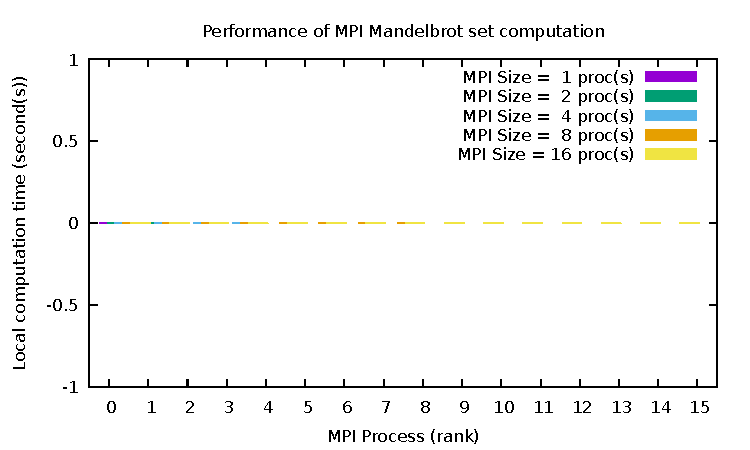
\includegraphics[scale = 1]{../04_mandel/perf.pdf}
    \caption{Performance of the parallel Mandelbrot set implementation.}
    \label{fig:mandelbrot_performance}
\end{figure}

A significant variability in execution time across processes can be observed. This is due to the intrinsic nature of the Mandelbrot set, where the number of iterations required for each pixel strongly depends on its position in the complex plane. Regions close to the boundary of the set require substantially more iterations, resulting in higher computational cost for the corresponding processes.\\

As a consequence, the workload is not uniformly distributed, and some processes complete their computation much earlier than others. This leads to load imbalance, which limits the overall parallel efficiency since the total execution time is determined by the slowest process.\\

Increasing the number of processes reduces the size of each subdomain but does not eliminate the imbalance. On the contrary, finer partitioning can make the variability more pronounced.\\

\subsection{Possible performance improvements}
Several strategies could be adopted to improve the performance of the MPI Mandelbrot implementation.\\

A first possible improvement concerns load balancing. The current block decomposition assigns each process one contiguous rectangular portion of the image. Since the Mandelbrot set is highly non-uniform, some subdomains contain many points close to the boundary of the set and therefore require significantly more iterations than others. This leads to processes with very different execution times. A better strategy would be to distribute the work in a more balanced way, for example by assigning rows or small tiles cyclically among the MPI processes. In this way, each process would receive a mixture of easy and expensive regions, reducing the imbalance.\\

Performance could also be improved by optimizing the local computation kernel. Since each process computes many independent pixels, the inner loops are good candidates for shared-memory parallelism through OpenMP, leading to a hybrid MPI+OpenMP implementation.\\

A further optimization would be to improve data locality and vectorization in the pixel computation loop. Careful restructuring of the computation, compiler optimization flags, and ensuring contiguous memory access patterns could help the compiler generate more efficient code.
\newpage
\section{Parallel matrix-vector multiplication and the power method
         [30 points]}


\end{document}


